\documentclass[10pt]{report}
\usepackage{graphicx}
\usepackage{a4}
\usepackage{url}
%\usepackage{fullpage}
%\usepackage{fancyhdr}

\setlength{\parskip}{0.3cm}
\setlength{\parindent}{0cm}

% This is the preamble section where you can include extra packages etc.

\begin{document}

\title{Report Two: Progress and Revisions}

\author{Corina Ciobanu \and Iskander Orazbekov \and Mir Sahin \and Paul Grigoras \and Radu Baltean-Lugojan}


\date{\today}         % inserts today's date

\maketitle            % generates the title from the data above

\begin{abstract}
This report presents a summary of the series of changes that our project has undergone and how we have adapted our work methodology in order to deliver agreed functionality on time, cope with the new requirements and minimize the negative impact on our application.
\end{abstract}

\tableofcontents

\renewcommand{\chaptername}{}

\chapter{Progress}
This section reports on the progress of the project, by detailing the accomplished features and important technical problems (and solutions) encountered so far.
\section{Iterations and Requirements}
Three iterations have been completed so far.

The table on page 4 details what features have been accomplished in each iteration, with the associated number of story points and version number.

On page 7, a screenshot of the application (version 0.3) has been included.

\section{Problems and Solutions}
A number of technical problems were generated by the unavailability of free tennis statistics. This has lead to an intricate and computationally intensive solution for obtaining the data, which in turn has lead to a shift towards a multi threaded architecture with all its associated complications.

All these issues have been overcome, as described in detail below, without significantly impacting the ability to deliver core functionality (and extensions) on time - a more detailed estimation is presented in sections \ref{schedule} and  \ref{estimating}.

\subsection{Dependencies on Third parties}
The lack of a central source for all the required data (market data, live scores and tennis statistics) has generated significant dependencies on external service providers. Furthermore, some data sources are very unreliable (e.g. data obtained by parsing web sites - as described in the next section).

The current solution is to design independent and resilient user interface components, such that if one fails or is delayed in fetching data, others remain functional and responsive.

\pagebreak
{\bf This page is intentionally left blank.}
\pagebreak

A long term solution aimed for iteration 8 is to move the logic for fetching live scores and tennis statistics (the major source of unreliability) to a remote server that provides a clean interface exposing all required data. Unfortunately, the Betfair certification program prevents us from additionally providing Betfair market data through this interface.

This architecture could offer an increase in performance and better stability for the desktop clients, but would add the complexity of another transport layer and also complicate the build process (since it would effectively lead to a separation into two projects).

\subsection{Lack of Free Tennis Statistics}
The unavailability of free data for player statistics has proven itself a major issue, forcing us to resort to data obtained from www.tennisinsight.com, by paying a small fee to get access to this comprehensive tennis statistics website. 

Though the method to fetch data is similar to the one employed in fetching live scores (detailed in Report One), additionally, we need to automatically execute some functionality of the website, like logging into our test account and navigating to the relevant player head-to-head comparison (for the currently selected match). This is achieved using the Rhino Engine included in HtmlUnit, which is able to natively execute Javascript and intercept its execution to collect data, allowing us to scrape the page we are interested in. Though the original intent of the HtmlUnit Java library is to unit test website builds, it can effectively be used to scrape information from live websites, mimicking the functionality of an automated headless browser. However, as detailed above, extensive data fetching poses more challenges to having a reliable and responsive application.

Obtaining this data is particularly important to the project because, aside from constituting a good source of information for the user, both live score and player statistics are to be used as inputs to a Markov chain model capable of accurately predicting live odds for the next point, set or entire match. This model will be integrated with our application and have all its outputs visible, as well as the predicted match odds displayed along the real ones on the graph. The user will thus be able to compare the prediction with the actual odds evolution and form opinions on possible trading arbitrage situations that may occur at any in-play time.

\subsection{The Switch to a Multi Threaded Architecture}
Because the task of fetching and parsing data is computationally intensive, as described above, we have decided to shift to a multi threaded architecture, splitting existing functionality into a user interface thread and a number of processing threads (responsible for fetching and processing data).

This architecture allows for a responsive user interface even in the (very likely) situation in which data is not available (e.g. if the network connection goes down) and is the foundation for the resilient and independent component model mentioned previously.

The separation achieved between user interface and logic should prove very  useful in iteration 8, facilitating the shift to the client server architecture.

\subsection{Threading Issues}

The shift to a multi threaded architecture has generated a few issues by itself.

The most significant one was related to the SWT threading model (apartment model), which does not allow updates of user interface components to be carried out from other threads than the user interface thread. This problem has been overcome through careful design, but required a more in depth understanding of the framework than we had initially anticipated.

Furthermore, it has become increasingly more difficult to reason about the correctness of the application (as in any multi threaded programs), which has led to an increased number of bugs. Although, so far, most have been rather obvious (e.g. hanging the user interface indefinitely), the team has decided to adopt more rigorous methods for spotting errors in order to prevent them from propagating to production code.
Namely, we intend to make even more use of pair programming, functional and unit testing in upcoming iterations.

Performance might also constitute an issue, particularly on single core, old generation CPUs. This concern has lead to the need for a more rigorous benchmarking approach, which should (at a minimum) provide some rough indicators of the performance of the application (number of threads, CPU utilisation, memory consumption, object instances etc). This is discussed in more detail in section \ref{perf}.

\subsection{Build Issues}

Currently the project uses a number of classes automatically generated from large WSDL specifications which are approximately 400 thousand lines long (just for the Betfair API).
This has generated a serious increase in compilation time due to some inefficiencies in the build script (e.g. a "run" performed a "clean" before recompilation).

Since the specifications are not expected to change often, the compiled classes have been packaged into a library, effectively removing the need for recompilation.
A task which automatically generates the classes, compiles, packages them and updates the library has benn added, should this be required in the future.

\pagebreak
{\bf This page is intentionally left blank.}
\pagebreak

\chapter{Revisions}

This section analyses changes and developments which have occured between the current status of the project and that at the time of the First Report.

It also includes a revised, less speculative schedule for future iterations (section \ref{schedule}).

\section{Requirements}

The set of requirements has been increased at the suggestion of our supervisor.
For example the ability to playback historical matches and record live data has been included, as described below.

\subsection{Key Requirements}
We have followed the initial strategy for most key features implemented in the project, making adjustments (time-wise and technical) where we either lacked resources or encountered technical issues. 

The first iteration comprised all the features we had planned for, such as setting up a login screen, score and graph displays and a navigation panel for a list of tennis matches. However, in iteration two, due to updates of score and player statistics, we switched to a multi-threaded architecture. 
As a side effect of threading issues similar to those in score fetching, the widget to display player statistics was implemented earlier. Though these statistics have the initial intended functionality, the underlying information source has changed to web scraping, due to the lack of any free online tennis API. 
Due to multi-threading, general UI, refactoring work and rapid advancement with the development of the graph display we decided to push back filtering and sorting matches down to milestone six.

A significant feature addition was adopting the Fracsoft playback of graph odds values, allowing us to display historical odds data by reading in .CSV files. This feature was originally suggested by our supervisor, but a library containing historical data had not been identified at that time, hence not included in our initial plan. As we added offline odds plotting with historical data, a recording of in-play odds and stats in the same format and an online/offline indicator are now considered requirements as well.

\subsection{Extensions}

Our extensions are in line with what we originally proposed, ideally aiming to provide both a virtual and a real betting environment for our user as well as a prediction model for spotting any market arbitrage opportunities. In addition, as a major performance improvement, a distributed architecture is considered as a last extension.

\section{Infrastructure Requirements}

It is possible that, for performance benchmarking (section \ref{perf}), we will require a number of different configuration PCs. Currently the application has been tested on 6 different machines (including dual core laptops and 2 quad core desktop configurations).

It is important to test the performance of the application on older generation PCs, preferably with single core CPUs and small memory size (e.g. 512 MB).

\section{Development methodology}

The team has decided to adopt a more rigorous development methodology, more aligned with Extreme Programming, as described in \cite{extremep}.
For this reason, a more specific set of practices will be adopted, which is expected to further improve productivity and communication between team members.

More rigorous estimation and performance measuring methods are also discussed.

\subsection{Practices}

A table summarizing the practices (as found in \cite{extremep}), whether they have been adopted or on course to be and the expected benefit or other observations is presented below. A number of practices are included in section \ref{manag}, so they are not covered here.

All practices should result in better cooperation and increased productivity so this is not included in the table.

{\bf Legend:}
\begin{description}
\item [Yes(n)] - applied beginning with iteration n 
\item [No(n)] - not yet applied, but should be applied no later than iteration n 
\end{description}

\begin{center}

\begin{tabular} {p{2.25cm}|p{4.5cm}|p{1.5cm}|p{5cm}}
{\bf Practice} & {\bf Short Description} & {\bf Applied} & {\bf Outcome / Observations}\\
\hline

Stories & "Plan using units of customer visible functionality" \cite{extremep} & Yes(0) & Providing earlier estimates would be beneficial. \\
\hline

Ten-Minute Build & Build the whole system and tests under 10 minutes. & Yes(0) \\
\hline

Continuous Integration & "Integrate and test changes after no more than a couple of hours." \cite{extremep} & No(5) & Helps identify errors or bugs  as soon as they are introduced.  \\
\hline

Test-First Programming & Write a failing automated test before changing any code. & No(4) & Helps avoid "scope creep"; improves coupling and cohesion;
improves trust and rhythm \\
\hline

Shared code & Any member can improve any part of the system at any time. &
Yes(2) & Risks include people acting irresponsibly (if they are not responsible for the particular piece of code) \\
\hline

Code and tests & Maintain only code and tests as permanent artifacts. & Yes(1) & Generate all documentation from code. \\
\hline

Single code base & There should be only one code stream and single branches shouldn't live for more than a few hours. & Yes(0) & A single master branch.
Only keep code for current release. \\
\hline

Daily Deployment & "Twelve releases sounds a lot better than twelve patches." (\cite{extremep}) & No(6) & Lack of continuous integration represents a technical barrier \\
\hline

Pay-per-Use & Charge every time the system is used & No(8) & Charge a base price for the application and then charge a small amount for individual widgets.

This provides good feedback on which widgets are actually useful/desired.

\end{tabular}

\end{center}

\subsection{Testing}

In terms of testing, particularly important are the "Test-First Programming" and "Continuous Integration" practices. These have not been applied so far due to lack of familiarity with testing APIs but also with other libraries. However, we have developed tests for the main classes, containing most of the business logic of our application.

After researching \cite{testing} and gaining a better understanding of the test-driven approach, we believe we have gained enough confidence to start  gradually applying the "Test-First Programming" practice, beginning with the next iteration.

Also, a continuous integration server will be deployed in the following iteration, since the application has reached a state in which errors can be easily introduced. This practice ensures any new bug can be quickly identified, at which point solving it becomes the priority - temporarily suspending other commits form taking place.

\subsection{Refactoring}

Refactoring has been applied frequently in order to improve code quality, which has lead to increased productivity. Most common applications such as method extraction have been at the heart of a continuous process which aimed to maintain code readability. Furthermore, large classes have been refactored to achieve decoupling between application logic and application UI.

A major redesigning of the code is intended to take place in iteration 4 in order to facilitate the introduction of the story "Record odds and data into .csv file" (Fracsoft format).

To ensure this progresses without breaking existing functionality, refactoring will be applied extensively.

\subsection{Planning and Estimating}
\label{estimating}
We are only using the primary indicators (described in Report One) as a reliable project measure - secondary indicators are just to give an overview of some important aspects of the project.
User satisfaction is high.
For measuring team velocity we take a moving averege of the last three iterations (as suggested in \cite{estim}), which leads to a velocity of 30. Further, we allow a margin for error, taking an interval around this average velocity which leads to the range 26-34 (\cite{estim}).

A burndown chart is used to rapidly indicate whether at the current velocity, the team is on schedule.

\begin{figure}[ht]
	\centering
	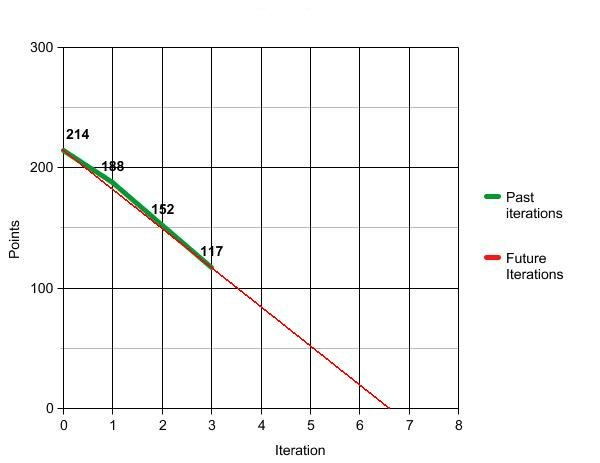
\includegraphics[bb= 0 0 400 400, scale=0.65]{graph.jpg}
	\caption{Burndown chart}
\end{figure}

Currently, we are expecting to finish before the begining of the 8th iteration, which allows additional time for unexpected issues, polishing or even addition of extra features.

\subsection{Benchmarking and Performance Measuring}
\label{perf}

As described above, because of the number of threads created by the application, it is important to test it on older generation, single core CPUs, which might experience a significant decrease in performance.

Currently we are researching into profiling tools such as the Eclipse Profiler, Netbeans Profiler, MemCheck, Cachegrind and the JVM Profiler Interface. These are aimed to help identify memory leaks and a number of runtime statistics (memory and cpu consumption, number of threads and object instances created, number of native objects created etc.). This is especially important due to the architecture of SWT, which, via native calls, creates instances which might not be garbage collected even at application shutdown.

It is hoped that profiling can be integrated with unit and functional testing by the end of iteration 5, creating the possiblity of running automated performance tests, which could, for example, start and close the application a large number of times asserting that memory consumption has not increased significantly.

\section{Schedule}
\label{schedule}

As explained above, all problems - technical or otherwise - have been overcome successfully, without significantly affecting our schedule. 

As in our initial draft schedule, the timescale of 8 weeks is divided into 8 iterations (we aim to complete a milestone and one iteration at the end of each week).
The first 5 weeks are mostly concerned with implementing the required features (including the new Fracsoft story), but due to reasons explained earlier we have also started work on some of the extensions.

The last 3 iterations aim at finishing the application final touches, as well as implementing as much as possible of the extensions.

The table on page 13 presents the revised schedule, indicating similarities and differences to the initial draft.

\pagebreak
{\bf This page is intentionally left blank.}
\pagebreak


\chapter {People Management}
\label{manag}

The goal of our group organisation is for everyone to contribute as much and as best as possible to the overall success of the project. 

\section{Managing Skill Set}

Since the application involves requirements from different areas (understanding tennis trading, studying a mathematical model for inferring probabilities, multi-threading) work among group members has been split according to each person's interests and experience. This ensures full use of members' up-to-date knowledge and an enthusiastic approach.

However, members' roles are not fixed, which allows everyone to contribute their best to the overall evolution of the project (e.g. persons interested in trading may also have very good UI design skills etc.).

\section{Managing Skill Levels}

GitHub issues are used to assign work among group members, each with a number of points to represent its difficulty and estimated time to solve. These provide us with the necessary data to monitor each person's work and rough contribution to the project (both in terms of completed issues, but also in terms of total time spent working on the project). 

Since our schedules are different (due to course options, coursework deadlines) we are interested in the long-term contribution of each member rather than a weekly analysis of the data. Hence, we consider the last 2-3 iterations when constructing these statistics, taking into account both the total time spent by each member and the overall difficulty of the solved problems. 

Although, ideally, we would want everyone to contribute equally, we think it is beneficial to everyone and to the project itself to encourage members to have initiative - propose improvements to the application and implement them.

\section{Practices}
To improve the team collaboration and maximise our productivity, we have adopted a number of practices(\cite{extremep}) in organising both our group meetings and some of our coding time:

\begin{description}
\item[Sit together] \hfill \\
	Regular meetings held in the labs, with all members of the team. These include discussion on the progress and current issues we are working on, but are mostly comprised of coding sessions. We have adopted this practice from Milestone 2 onwards.
\item[Informative Workspace] \hfill \\
	Before coding started, regular meetings were held in the library, making use of the projector and board to create our own development / planning room. Due to the lack of an actual space dedicated to our team, we are currently using a portable white board to stick and write current issues on.
\item[Energized work] \hfill \\
	Work is only done when high productivity can be achieved. The Github punchcard history has proved very useful in identifying the days and times of the week when highest productivity has been achieved.
\item[Weekly cycle] \hfill \\
	The weekly cycle corresponds to the weekly iteration. Every cycle we review our progress and compare it to our estimation and plan the stories for next iteration - considering the suggestions of our client (supervisor) and our estimated velocity based on the previous three iterations. Since \emph{ownership of tasks} is also one of the important practices we use, stories are broken into several tasks, for which members sign up or are assigned to, taking full ownership of the issue.
\item[Pair Programming] \hfill \\
Frequently, some of the issues are assigned to two members of the team, which work together to solve them. This mostly includes pair programming, with two people sitting at one machine and solving one problem. So far, this practice has yielded very good results in solving several difficult issues (e.g. switching to a multi-threading architecture).

\end{description}

Also, since our project requires some investments (e.g. Fracsoft files, Betfair API access etc.) a group budget has been created to which all members contribute equally.

\section{Solving Problems \cite{teamdysf}}

As different problems may arise throughout the project, we have created from the beginning a strong team, capable of arguing about different issues and reaching a solution in the best interest of the application and of the group. Hence we are focusing on constantly building trust among ourselves, so that we feel comfortable arguing about any possible problem and able to fully commit to finding its best solution - focusing on the overall result of the team and the application rather than on individual goals or desires.

\chapter {Ethical and Environmental Impact}

\section {Ethical Issues}

It is important to note that Tennis Trader is intended for an audience of  traders which (similarly to, for example, traders in banks) are trained professionals with a good understanding of their risk exposure and with a calculated profit strategy.

Nevertheless, the application is - ultimately - intended to be used by people to bet on the outcome of a tennis match or to speculate on the fluctuation of the betting odds (tennis trading), which constitute serious forms of gambling, presenting complex issues in terms of ethics and addiction.

\subsection {Gambling}

As statistics show that it is more likely for a person to gamble online than at a regular bookmaker \cite{onlngamb}, the platform presents a risk for people with a gambling addiction because of the ease and convenience of using it on any Internet connected PC  from any location in the world. Furthermore, since a user will be able to login with their Betfair account, the feature to fund the account through online bank transactions and credit cards will be available, which further facilitate addictive online gambling.  

In the UK, gambling is regulated by the UK Gambling Commission. Consequently, the product must adhere to a set of requirements prior to commercialization (\cite{betfappcert, betfreq}) which interdict, for example, active encouragement of players (e.g. to try to win back their losses or to continue playing etc.).

Furthermore, the application is required to respect Betfair�s Advertising and Marketing Guidelines \cite{betfadv}. 

All these requirements are set to protect addicts and to combat ethical issues related to gambling. 

At the moment a user cannot place a bet, but in implementing this feature we will ensure that we satisfy all the necessary requirements (e.g. by clearly displaying the gambling content, not encouraging clients to recover their losses etc). 
When our application will be ready for advertising, we will take into account Betfair�s Advertising and Marketing Guidelines and none of our advertising materials will hide the risk of gambling. 

\subsection {Age Regulation}

Another source of concerns is the age regulation imposed on gamblers, as it is often impossible to identify the age of a user, potentially allowing underage persons to use the application.
To be able to use the application a user will need to have a Betfair account where he/she upon creation must accept a set of Terms and Conditions which clearly specify the circumstances of illegal use. Furthermore, Betfair does not allow bet placing until the user has confirmed his age by making a transaction with a credit card (which are only emitted to people over 18).
Because all transactions are executed through the Betfair API, it will not be possible for an underage person to place bets.

Additionally, Tennis Trader will come with a very strict set of Terms and Conditions, clearly stating that betting is highly addictive and that the use of our platform is only permitted to over 18. 

Furthermore if a user is suspected of misuse or any other fraudulent behaviour, Betfair and the regulation agencies will be informed promptly.

\subsection {Personal Data}

Another ethical issue is concerned with handling of personal data. Since the Betfair API is quite permissive, it is possible to access a significant amount of the user�s personal data, stored in the Betfair account.
Currently the application does not offer a means of viewing or editing this data, but in the future, it is important to ensure that all precautionary measures are taken as described by the Data Protection Act[6].

Furthermore, in order for the application to be available commercially, it must pass Betfair�s certification process, which enforces a set of security requirements such as direct communication with Betfair API, no automatic login, storage of username only if encrypted and invisibility of any other user�s sensitive data from vendor. 

We are aware of all security requirements and during the development of our application we will ensure that these are implemented, in order to avoid failing the Betfair certification process. 

\subsection {Licenses}

Currently, the project depends on a number of open source libraries and it is vital to ensure that every one of them has a license which permits selling the application and if not, that it is replaced.

Strictly speaking, since selling the application is a long term goal (past January 2011) and on the short term (December) the team is focused on delivering a good, functional (academic) project, we have decided to use even libraries which may not have a very permissive license - with the aim of replacing them in the future - in order to speed up the development process.

\section {Environmental Impact}

Initially the project was considered to be distributed either on CDs or via on-line download. However the environmental concerns connected to the production of CDs and their packaging (recycling of the polycarbonate plastic used in the production of CDs is not available world-wide) led to the latter option being preferred.

Furthermore, most of the competing software packages in this niche are distributed on-line, reducing potential environmental impact and also increasing cost effectiveness.

The web application required for distribution is not expected to have a high CPU demand, providing limited functionality such as user registration, online payment, documentation, user guides and FAQs.

However, it will provide the ability download the application which is expected to require a large bandwidth.
The rather narrow audience for which the application is targeted implies a small number of downloads is expected on average, with increases in demand likely to occur at the time of new releases or patches to the older versions.
The size of the download is projected to be around 50 MB, assuming the Java Runtime Environment is not included. 
Taking this into account, the project will not need a very powerful server, leading to a reduced environmental footprint.

The desktop application itself has high CPU requirements, but not as much as, for example, graphically demanding applications (high end CPU consumption is on average 2-3 times smaller than high end graphics cards).

Finally, the impact of the server program which will be created in iteration 8 for score and live statistics fetching should be included. The migration to a client server architecture should in fact reduce power consumption since CPU intensive (and power hungry) data fetching and processing are only carried out by a single machine (the server) and not all the clients.

Overall, the environmental impact is expected to be relatively modest and can be reduced further only by deploying more power efficient code. This can be achieved with the help of the compiler (optimizing for power consumption) or by reducing the complexity of the computations (e.g. by using quicksort, binary search, hash maps etc.).

\chapter {Conclusions}

In spite of good progress in the first three iterations, the team has adopted a more rigorous work methodology (more aligned to Extreme Programming) as well as a more established method for estimating and planning (based on story points, velocity, burndown charts). 
This is expected to increase productivity and provide a more accurate indication of the team�s ability to finish the project on time.

A number of substantial technical problems have been overcome without significantly affecting the chances of delivering core functionality on time.

A number of ethical, legal and environmental issues with potential technical impact on the project have been analysed and taken into account in redesigning the plan for future iterations.
 

\begin{thebibliography}{9}

\bibitem{extremep}
	Kent Beck with Cynthia Andres,
	\emph{Extreme Programming Explained Second Edition: Embrace Change},
	Addison-Wesley,
	2004

\bibitem{estim}
	Mike Cohn,
	\emph{Agile Estimating and Planning},
	Prentice Hall,
	June 2010

\bibitem{refact}
	Joshua Kerievsky,
	\emph{Refactoring to Patterns},
	Addison-Wesley,
	2004

\bibitem{testing}
	Steeve Freeman, Nat Pryce,
	\emph {Growing Object-Oriented Software, Guided by Tests}
	Addison-Wesley
	2010

\bibitem{onlngamb}
	Adrienne Welch and Danielle Crowle,
	\emph{�Types of online gambling and the ethics of the issue�}, \hfill \\
\url{http://www.uri.edu/personal/awel5922/gambling.index.html}

\bibitem{betfappcert}
	\emph{Betfair Vendor Application Certification; Part B: Product Requirements}, \hfill \\
\url{http://bdp.betfair.com/index.php?Itemid=58\&id=76\&option=com\_content\&task=view}

\bibitem{betfreq}
\emph{Betfair Gambling Commission - Remote Gambling and Software Technical Standards Requirements}, \hfill \\
\url{http://bdp.betfair.com/index.php?option=com\_content\&task=view\&id=69\&Itemid=59} 

\bibitem{betfadv}
	\emph{Betfair Advertising and Marketing Rules}, \hfill \\
\url{http://bdp.betfair.com/images/stories/betfair/sports/documentation/BetfairAPISoftwareVendorAdvertisingRules.pdf}

\bibitem{dataprot} 
	\emph{Data Protection Act 1998} \hfill \\
\url{http://www.legislation.gov.uk/ukpga/1998/29/contents}

\bibitem{teamdysf}
 Patrick Lencioni,
 \emph{Overcoming the Five Dysfunctions of a Team: A field guide}

\bibitem{agilesam}
	Jonathan Rasmusson,
	\emph{The Agile Samurai},
	Pragmatic Bookshelf,
	October 2010.

\bibitem{}
	Jeff Langr and Tim Ottinger,
	\emph{Agile in a Flash},
	Pragmatic Bookshelf, 
	January 2011.

\bibitem{}
	\emph{Robert Chatley's course on Software Engineering Methods}  \hfill \\
	\url{http://www.doc.ic.ac.uk/~rbc/302/}, 
	Imperial College London


\end{thebibliography}

\end{document}
